\documentclass[svgnames]{beamer}


% \usepackage{mathtext}
\usepackage[utf8]{inputenc}
\usepackage[english,russian]{babel}
\usepackage{cmap}
\hypersetup{unicode=true}
\graphicspath{{images/}{slides/images}}


\title[CMTA 04] % (optional, use only with long paper titles)
{Vector space model}

\subtitle
{Computational Methods for Text Analysis} % (optional)

\author%[Author, Another] % (optional, use only with lots of authors)
{Pestova Alena}
% - Use the \inst{?} command only if the authors have different
%   affiliation.

\institute%[Universities of Somewhere and Elsewhere] % (optional, but mostly needed)
{HSE Saint-Petersburg}
% - Use the \inst command only if there are several affiliations.
% - Keep it simple, no one is interested in your street address.

\date%[Short Occasion] % (optional)
{04.10.2021}

\subject{natural language processing, text mining}
% This is only inserted into the PDF information catalog. Can be left
% out.


%\AtBeginSubsection[]
%{
%  \begin{frame}<beamer>[plain]{План}
%    \tableofcontents[sectionstyle=show/hide,subsectionstyle=show/shaded/hide]
%  \end{frame}
%}

\newcommand{\tb}[1]{\colorbox{yellow}{#1}\space}
\newcommand{\Sp}[1]{\colorbox{green}{#1}\space}
\newcommand{\Sn}[1]{\colorbox{red}{#1}\space}


\begin{document}

\begin{frame}
  \titlepage
\end{frame}


\begin{frame}{Vector space model: bag of words}

  \begin{block}{For statistical analysis we need a transformation:}
      Text $\longrightarrow$ Set of features
  \end{block}

  \begin{itemize}
  \item Each word of the text [type] — свойство
  \item Word Frequency - a value of the feature
  \end{itemize}

    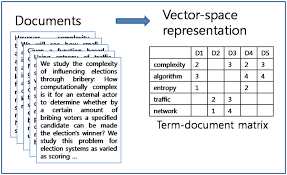
\includegraphics[height=.4\textheight]{dtm}
\end{frame}


\begin{frame}
    Why do we need to transoform documents to vectors?
    \begin{itemize}
        \item to compare them, to separate them into groups
        \item for classification
        \item many other tasks
    \end{itemize}
\end{frame}

\begin{frame}[fragile]
  \frametitle{Document Vector Representation}
  \small
  \begin{block}{}
    - Мне, пожалуйста, двойной виски. - Девочка! Это школьная
    столовая! - Ой, извините, я задумалась. Компот, пожалуйста...
  \end{block}
  \footnotesize
\begin{verbatim}
виски    двойной    девочка задумалась   извините
    1          1          1          1          1
компот        мне   пожалуйста     столовая     школьн
     1          1            2            1          1
это
  1
\end{verbatim}
\end{frame}

%\subsection{Vectors in multidimensional space}
%
%\begin{frame}
%  \frametitle{Вектор}
%  \begin{columns}
%    \column{.5\textwidth}
%    \begin{tabular}{ccc}
%      \only<2->{ russian & maths & physics \\
%        \hline}
%      90 & 60 & 90 \\
%      \only<3->{
%        95 & 65 & 95 \\
%        67 & 98 & 100 \\
%      }
%    \end{tabular}
%    \column{.5\textwidth}
%\only<4>{
%    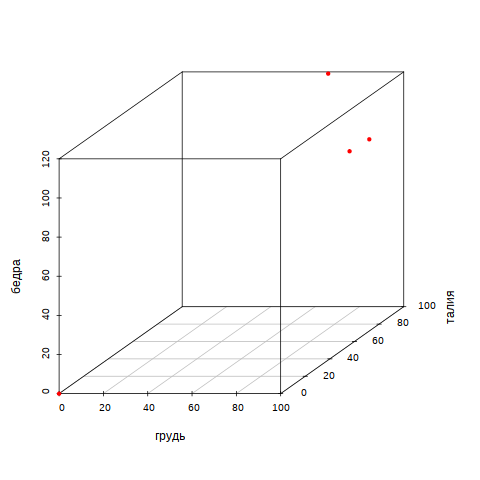
\includegraphics[width=\textwidth]{vectors0}
%}
%  \end{columns}
%\end{frame}
%
%\begin{frame}
%  \frametitle{Similarity of vectors: Euclidean distance}
%  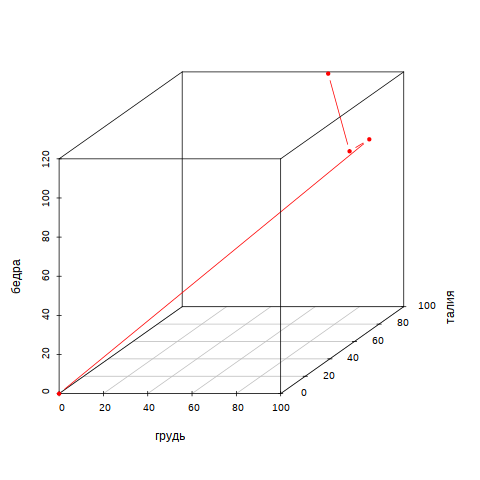
\includegraphics[height=.9\textheight]{vectors1}
%\end{frame}
%
%\begin{frame}
%  \frametitle{Similarity of vectors: cosine distance}
%\only<1>{
%  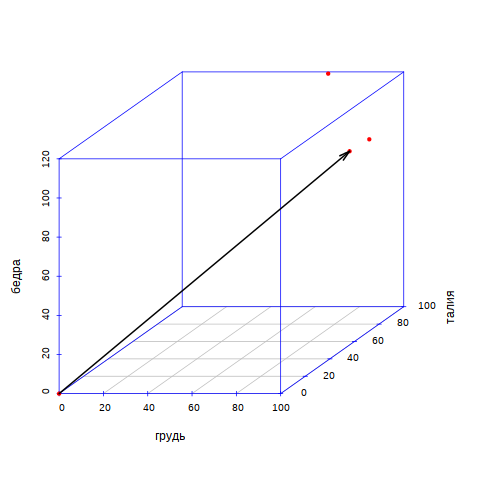
\includegraphics[height=.9\textheight]{vectors2}
%}
%\only<2>{
%  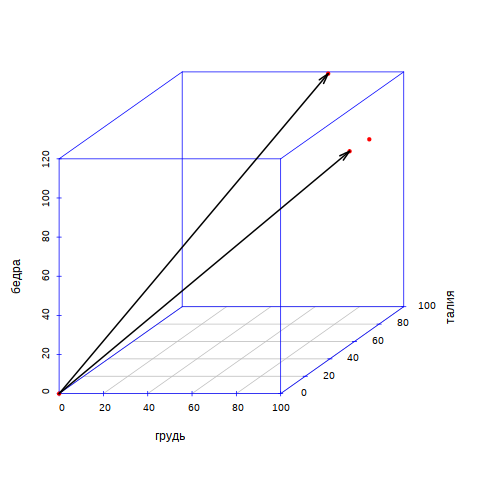
\includegraphics[height=.9\textheight]{vectors3}
%}
%\end{frame}

\begin{frame}
  \frametitle{Measures of distance}
  Similarity of documents = vectors similarity (in N-dimensional space)
  \begin{itemize}
  \item Euclidean distance $L_2(x,y) = \sqrt{\sum_{i=1}^{m}(x_i-y_i)^2}$
  \item $L_1(x,y) = \sum_{i=1}^{m}|x_i-y_i| $
  \item cosine distance $\frac{x\cdot y}{|x|\cdot|y|} = 1 -
    \frac{\sum_{i=1}^{n}(A_i\times B_i)}{\sqrt{\sum_{i=1}^{n}(A_i)^2}\sqrt{\sum_{i=1}^{n}(B_i)^2}}$
  \item cosine similarity  $1-\frac{x\cdot y}{|x|\cdot|y|}$
  \end{itemize}
\end{frame}



\begin{frame}[fragile]
  \frametitle{Document-term matrix}
  Terms with the highest DF (document frequency)
  \footnotesize
\begin{verbatim}
Docs вовочк дет класс урок учител учительниц школ
   1      2   0     0    1      0          1    0
   2      2   0     0    0      0          1    0
   3      1   1     0    0      0          1    2
   4      3   1     0    1      0          1    0
   5      3   0     0    0      0          1    0
   6      1   0     0    0      0          1    0
\end{verbatim}
\end{frame}



\begin{frame}
  The frequency matrix describes the observed intersections of two
   sets:
   \begin{itemize}
   \item set of allowed words (types)
   \item set of valid text objects
   \end{itemize}
\end{frame}

\begin{frame}{Document frequency}
    \begin{itemize}
  \item We can just take the document frequency of each word and put to the matrix
  \item The problem - the length of documents varies greatly
  \item The second problem - not all words characterize the document (stop-words and just common words)

\end{itemize}
    \end{frame}

\begin{frame}{Vocabulary}
  By defining a fixed dictionary, we define the features , within which our
  documents can be described.

  For example, in Shakespeare:

  \begin{description}
  \item[ipad] there were no such a word (there is no sense in including it)
  \item[theology] could have used (as some him contemporaries do), but
    did not use
  \item[christ] never used this word in comedies, but
    used in several historical plays
  \end{description}
\end{frame}


\begin{frame}
  \frametitle{Distribution of vocabulary across documents}
  \begin{itemize}
  \item Frequency reflects the importance of the word in the language/document collection
  \item But it strongly depends on the composition of the collection, (for ex: mean word frequency \alert{hobbit})
  \item In addition to frequency, \alert{dispersion} needs to be taken into account —
    how evenly the word is distributed across the documents
  \end{itemize}
\end{frame}



\begin{frame}
  \frametitle{IDF: inverse document frequency}
  \begin{equation}
    IDF=\log_2\frac{D}{df}
  \end{equation}
  где
  \begin{itemize}
  \item[$D$] — the number of documents in the corpus
  \item[$df$] — the frequency of the word in the collection of documents
  \end{itemize}
\end{frame}

\begin{frame}
  \frametitle{IDF: примеры}
  \begin{tabular}[l]{lccc}
    распределение & D & df & IDF \\
    \hline
    везде & 10000 & 10000 & 0 \\
    часто & 10000 & 1000 & 3,32 \\
    достаточно & 10000 & 100 & 6,64 \\
    несколько & 10000 & 10 & 9,96 \\
    в одном документе & 10000 & 1 & 13,29 \\
  \end{tabular}
\end{frame}


\begin{frame}
  \frametitle{Correction for variance}
  Idea: adjust the ranking in the frequency list in
  according to dispersion. Tasks:
  \begin{description}
  \item[information search] lower the rank of words distributed  evenly

    The goal is to increase the rank of words that distinguish individual documents.

  \item[frequency dictionaries] lower the rank of words allocated unevenly

    The goal is to lower the rank of words that received an unreasonably high
    frequency due to the composition of the case.
  \end{description}
\end{frame}

\begin{frame}
  \frametitle{TF-IDF}
  Term-frequency-inversed document frequency - is a numerical statistic that is intended to reflect how important a word is to a document in a collection or corpus.
  \begin{equation}
    TF \times IDF = tf\log_2\frac{D}{df}
  \end{equation}
  \begin{itemize}
  \item[$tf$]  term frequency - is the relative frequency of term t within document d (raw count of a term in a document / the total number of terms in document)
  \item[$df$] document frequency - the frequency of the word in the collection of documents
  \item $\frac{D}{df}$ inverse document frequency - a measure of how much information the word provides, i.e., if it is common or rare across all documents.
  \item[$D$] the number of all documents in the corpus
  \end{itemize}
\end{frame}


\begin{frame}
  \frametitle{Weighing Terms}
  Words should \alert{distinguish} documents:
  \begin{itemize}
  \item not too frequent (uninformative, do not allow to separate
    various documents)
  \item are not too rare (do not allow similar documents to be combined)
  \end{itemize}
\end{frame}

%\begin{frame}[fragile]
%  \frametitle{Normalizing by text lengr}
%  Нормализация: разделить каждое значение на количество слов в документе
%  \footnotesize
%\begin{verbatim}
%    Terms
%Docs    вовочк       дет класс      урок учител учительниц школ
%   1 0.5000000 0.0000000     0 0.2500000      0  0.2500000  0.0
%   2 0.6666667 0.0000000     0 0.0000000      0  0.3333333  0.0
%   3 0.2000000 0.2000000     0 0.0000000      0  0.2000000  0.4
%   4 0.5000000 0.1666667     0 0.1666667      0  0.1666667  0.0
%   5 0.7500000 0.0000000     0 0.0000000      0  0.2500000  0.0
%   6 0.5000000 0.0000000     0 0.0000000      0  0.5000000  0.0
%\end{verbatim}
%\end{frame}

\begin{frame}[fragile]
  \frametitle{TF-IDF}
  Normalization: instead of simple word count (DF) we can weighted frequency  (TF-IDF)
  \footnotesize
\begin{verbatim}
    Terms
Docs    вовочк       дет класс      урок учител учительниц      школ
   1 0.6897996 0.0000000     0 0.4192463      0  0.4022703 0.0000000
   2 0.9197328 0.0000000     0 0.0000000      0  0.5363604 0.0000000
   3 0.2759198 0.4781918     0 0.0000000      0  0.3218162 0.4736512
   4 0.6897996 0.3984932     0 0.2794975      0  0.2681802 0.0000000
   5 1.0346994 0.0000000     0 0.0000000      0  0.4022703 0.0000000
   6 0.6897996 0.0000000     0 0.0000000      0  0.8045405 0.0000000
\end{verbatim}
\end{frame}

\begin{frame}[fragile]
  \frametitle{Cosine distance}

  \footnotesize
\begin{verbatim}
> dissimilarity(sp, method="cosine")
          1          2         3         4          5
1 0.0000000 0.11461112 0.5542388 0.1226977 0.12552228
2 0.1146111 0.00000000 0.4965362 0.1747931 0.01232358
3 0.5542388 0.49653624 0.0000000 0.3369433 0.53009027
4 0.1226977 0.17479311 0.3369433 0.0000000 0.16449672
5 0.1255223 0.01232358 0.5300903 0.1644967 0.00000000
\end{verbatim}

%  \footnotesize
%\begin{verbatim}
%Docs вовочк дет класс урок учител учительниц школ
%   1      2   0     0    1      0          1    0
%   2      2   0     0    0      0          1    0
%   3      1   1     0    0      0          1    2
%   4      3   1     0    1      0          1    0
%   5      3   0     0    0      0          1    0
%\end{verbatim}

\end{frame}


\end{document}
